\documentclass[a4paper, 12pt]{article}

\newcommand\tab[1][.6cm]{\hspace*{#1}}
\usepackage[portuges]{babel}
\usepackage[utf8]{inputenc}
\usepackage{amsmath}
\usepackage{indentfirst}
\usepackage{graphicx}
\usepackage{multicol,lipsum}
\usepackage{blindtext}
\usepackage{verbatim}
\usepackage{textcomp}
\usepackage{hyperref}
\usepackage{float}
\usepackage{url}
\usepackage{wrapfig}
\usepackage{lscape}
\usepackage{rotating}
\usepackage{epstopdf}

\begin{document}
%\maketitle

\begin{titlepage}
	\begin{center}
	
	\begin{figure}[ht]
    \centering
    
\includegraphics[width=.44\textwidth]{Images/LogoUFSJ.PNG}
    \label{fig:Capturar.PNG}
    \end{figure}

    	\Huge{Universidade Federal São João del-Rei}\\
		\Large{Curso de Ciência da Computação}\\ 

        \vspace{82pt}
        \textbf{\LARGE{
        \\
        \\
        \\
        Trabalho Prático - Parte 3\\
        Implementação do Sistema\\
        \vspace{0.5cm}
        \Large{Banco de Dados}
        \\
        \\
        \\
        }}
        
		\title{{\large{Título}}}
		\vspace{1cm}
	\end{center}
	    
    \begin{flushleft}
		\begin{tabbing}
		\\
		\\
		\\	
		\large{Discentes: Júlio César Ferreira,}\\ 
		\large{\hspace{2.35cm}Elias De Paula Pereira},\\
		\large{\hspace{2.35cm}Patrick Leandro Magalhães},\\
		\large{\hspace{2.35cm}Juan Victor Costa Silva Aleixo} e\\
		\large{\hspace{2.35cm}Julio Cesar da Silva Rodrigues}\\
	    \\
		\large{Docente: Leonardo Chaves Dutra da Rocha}\\
	    \end{tabbing}
    \end{flushleft}
	\vspace{0.8cm}
	
	\begin{center}
		\vspace{\fill}
			Dezembro\\
		    2022
	\end{center}
\end{titlepage}

\tableofcontents
\newpage

\section{Introdução}

Neste documento, serão apresentados de forma detalhada, os aspectos envolvidos nas modificações e correções realizadas nos modelos conceituais para modelagem de um banco de dados para uma rede de hotéis, cujo desenvolvimento foi iniciado na primeira parte do trabalho prático.

Serão abordadas as moficações mais cruciais e relevantes exploradas nos modelos de Entidade-Relacionamento Estendido e Relacional, a implementação atual do banco de dados de forma geral, funcionalidades presentes no sistema, limitações e também outros aspectos relacionados a requisitos não funcionais, como dependências funcionais e normalização.

\section{Modificações nos Modelos Conceituais}

Nesta seção, serão abordadas entidades, relacionamentos e seus respectivos atributos que sofreram quaisquer modificações, assim como as respectivas restrições de domínio que foram analisadas na construção dos modelos conceituais do banco de dados.

\subsection{Modelo Entidade-Relacionamento Estendido}

À seguir é apresentada por extenso a composição geral do modelo EER, contendo suas entidades, respectivos atributos e cada restrição de domínio correspondente:

\begin{itemize}
    \item \emph{\large Usuário}
    \begin{itemize}
        \item \textbf{Login}: Atributo do tipo \emph{String} com 45 caracteres variável;
        \item \textbf{Senha}: Atributo do tipo \emph{String} com 45 caracteres variável;
        \item \textbf{CPF}: Atributo do tipo \emph{Integer}, único com 11 caracteres;
        \item \textbf{Primeiro\_nome}: Atributo do tipo \emph{String} com 45 caracteres variável;
        \item \textbf{Sobrenome}: Atributo do tipo \emph{String} com 45 caracteres variável;
        \item \textbf{Datanascimento}: Atributo do tipo \emph{Date} (AAAA-MM-DD);
        \item \textbf{Telefone}: Atributo do tipo \emph{Integer} com 11 caracteres;
        \item \textbf{Endereço}: Atributo do tipo \emph{String} com 45 caracteres variável;
        \item \textbf{Email}: Atributo do tipo \emph{String} com 45 caracteres variável;
        \item \textbf{Diárias}: Atributo do tipo \emph{Integer} variável.
    \end{itemize}
    
    \item \emph{\large Dependente} (Entidade Fraca)
    \begin{itemize}
        \item \textbf{CPF}: Atributo do tipo \emph{Integer}, único com 11 caracteres;
        \item \textbf{Primeiro\_nome}: Atributo do tipo \emph{String} com 45 caracteres variável;
        \item \textbf{Sobrenome}: Atributo do tipo \emph{String} com 45 caracteres variável;
        \item \textbf{Datanascimento}: Atributo do tipo \emph{Date} (AAAA-MM-DD).
    \end{itemize}

    \item \emph{\large Hotel}
    \begin{itemize}
        \item \textbf{Cod\_hotel}: Atributo do tipo \emph{Integer}, único e de tamanho variável;
        \item \textbf{Localizacao}: Atributo do tipo \emph{String} multivalorado;
        \item \textbf{Nome}: Atributo do tipo \emph{String} com 45 caracteres variável.
    \end{itemize}

    \item \emph{\large Quarto}
    \begin{itemize}
        \item \textbf{Número}: Atributo do tipo \emph{Integer}, único e de tamanho variável;
        \item \textbf{Descrição}: Atributo do tipo \emph{String} com 45 caracteres variável;
        \item \textbf{Tipo}: Atributo do tipo \emph{String} com 45 caracteres variável (Standard, Luxo, Premium, ...);
        \item \textbf{Capacidade}: Atributo do tipo \emph{Integer} variável;
        \item \textbf{Status}: Atributo do tipo \emph{Boolean} que indica se o quarto está ou não ocupado.
    \end{itemize}
    
    \item \emph{\large Reserva}
    \begin{itemize}
        \item \textbf{Cod\_reserva}: Atributo do tipo \emph{Integer}, único com 11 caracteres;
        \item \textbf{Valor\_total}: Atributo do tipo \emph{Double} variável;
        \item \textbf{Valor\_desconto}: Atributo do tipo \emph{Integer} variável;
        \item \textbf{Feriado}: Atributo do tipo \emph{Boolean} para indicar reservas realizadas em período de feriado;
        \item \textbf{Estado}: Atributo do tipo \emph{String} com 9 caracteres \{'reservado', 'hospedado', 'cancelado'\};
        \item \textbf{Data\_inicial}: Atributo do tipo \emph{Date} (AAAA-MM-DD);
        \item \textbf{Data\_final}: Atributo do tipo \emph{Date} (AAAA-MM-DD);
        \item \textbf{Num\_ocupantes}: Atributo do tipo \emph{Integer} variável.
    \end{itemize}
    
\pagebreak

    \item \emph{\large Cupom}
    \begin{itemize}
        \item \textbf{Cod\_cupom}: Atributo do tipo \emph{Integer} variável;
        \item \textbf{Status}: Atributo do tipo \emph{Boolean} para identificar se o cupom é válido ou não;
        \item \textbf{Valor\_desconto}: Atributo do tipo \emph{Integer} variável.
    \end{itemize}

    \item \emph{\large Feriado}
    \begin{itemize}
        \item \textbf{Cod\_feriado}: Atributo do tipo \emph{Integer}, único com 11 caracteres;
        \item \textbf{Nome}: Atributo do tipo \emph{String} com 45 caracteres (variável);
        \item \textbf{Data\_inicial}: Atributo do tipo \emph{Date} (AAAA-MM-DD);
        \item \textbf{Data\_final}: Atributo do tipo \emph{Date} (AAAA-MM-DD).
    \end{itemize}

\end{itemize}

\noindent Os relacionamentos presentes neste modelo EER são sumarizados à seguir:

\begin{itemize}
    \item \emph{DEPENDENTES\_DE}: Relação entre Dependente e Usuário. Um usuário pode possuir múltiplos dependentes (\(1:N\)). Dependente possui participação total, pois todo dependente deve estar obrigatoriamente relacionado a um usuário. Usuário possui participação parcial, já que este pode ou não ter dependentes associados. É um relacionamento de identificação, visto que Dependente é uma entidade fraca.
    \item \emph{TRABALHA\_EM}: Relação entre Administrador e Hotel. Cada hotel possui um administrador (\(1:1\)). Participação total de ambas as entidades, pois todo administrador deve estar associado à um hotel e todo hotel deve possuir um administrador.
    \item \emph{CATALOGA}: Relação entre Administrador e Feriado. Um administrador pode cadastrar múltiplos feriados (\(1:N\)). Feriado possui participação total, pois todo feriado deve ser catalogado por um administrador, enquanto administrador tem participação parcial, já que este pode ou não catalogar feriados.
    \item \emph{GANHA}: Relação entre Cupom e Cliente. Um cliente pode ganhar múltiplos cupons (\(1:N\)). Participação parcial de ambas as entidades, pois nem todo cliente terá cupons e o cadastro de um cupom não depende da existência de um cliente.
    \item \emph{REALIZA}: Relação entre Cliente e Reserva. Um cliente pode realizar múltiplas reservas (\(1:N\)). Reserva possui participação total, pois toda reserva deve obrigatorimente estar relacionada à um cliente para existir. Cliente possui participação parcial, já que este pode ou não possuir reservas associadas ao seu CPF.
    \item \emph{VINCULA}: Relação entre Cupom e Reserva. Uma reserva pode ter múltiplos cupons associados (\(1:N\)). Reserva possui participação parcial, pois não é necessário que toda reserva esteja associada à um cupom, enquanto cupom também possui participação parcial, já que este pode existir sem que esteja vinculado à uma reserva (cupom ainda não utilizado).
    \item \emph{POSSUI}: Relação entre Hotel e Quarto. Um quarto deve estar associado à um único hotel até por questões físicas, e não deve existir sem que esteja associado ao mesmo. Hotel também possui participação total, pois todo hotel deve estar associado à pelo menos um quarto em sua existência (\(1:N\)).
    
\end{itemize}

\subsubsection{Observações}

Usuário pode assumir papéis de cliente e/ou administrador de forma conjunta (\emph{overlapped}) se aplicável. Por exemplo, um administrador pode atuar como cliente em ocasiões não habituais (um administrador que está de folga e realizou uma reserva como cliente no hotel em que trabalha), com ambos papéis herdando da entidade \emph{Usuário}.

Além disto, existem algumas entidades e relacionamentos presentes (assim como seus atributos) no modelo inicial que optamos por remover do modelo conceitual final para o banco de dados. Estas são exibidas na Tabela \ref{tab:exampleTab1}:
\begin{table}[H]
    \centering
    \caption{Entidades e Relacionamentos Removidos}\vspace{0.5cm}
    \label{tab:exampleTab1}
    \begin{tabular}{c|c}
        \textbf{Entidade} & \textbf{Relacionamento}\\
        Fornecedor & FF\\
        Produto & FP\\
        Fornece & FH
    \end{tabular}
\end{table}

Os obstáculos encontrados ao lidar com estas entidades foram de que, primeiramente, um \emph{fornecedor} era tratado obrigatoriamente como um usuário previamente cadastrado no sistema do \emph{hotel} correspondente, o que não necessariamente é aplicável na prática. Também foram encontradas dificuldades quanto ao gerenciamento da complexidade de representar tais entidades e relacionamentos como tabelas no banco de dados, no que diz respeito a implementação das funcionalidades básicas e geração de relatórios.

Algumas outras modificações também foram realizadas como a adição de um relacionamento entre \emph{Reserva} e \emph{Cupom} (\emph{VINCULA}), para que um usuário seja capaz de utilizar seus cupons. \emph{Quarto} agora possui relacionamento com \emph{Hotel} diretamente em vez de \emph{Reserva} por questões de consistência, já que a existência de quartos não depende da existência de reservas, e sim de hotel, transferindo a lógica de cadastro de reservas para a aplicação (e.g., valor conforme o tipo de quarto).

Por fim, foram adicionados os atributos correspondentes à capacidade dos quartos e número de ocupantes da reserva, para manter a consistência com as capacidades máximas de cada quarto na realização de reservas. O atributo \emph{Salario} foi removido da entidade \emph{Administrador}, assim como seu relacionamento com \emph{Cupom} (O administrador ainda é capaz de inserir cupons, apenas não existe referência a qual destes fez o cadastro).

A representação ilustrativa do modelo Entidade-Relacionamento Estendido é exibida na página \pageref{fig:exampleFig1} na Figura \ref{fig:exampleFig1}.

\begin{sidewaysfigure}[ht]
    \centering
    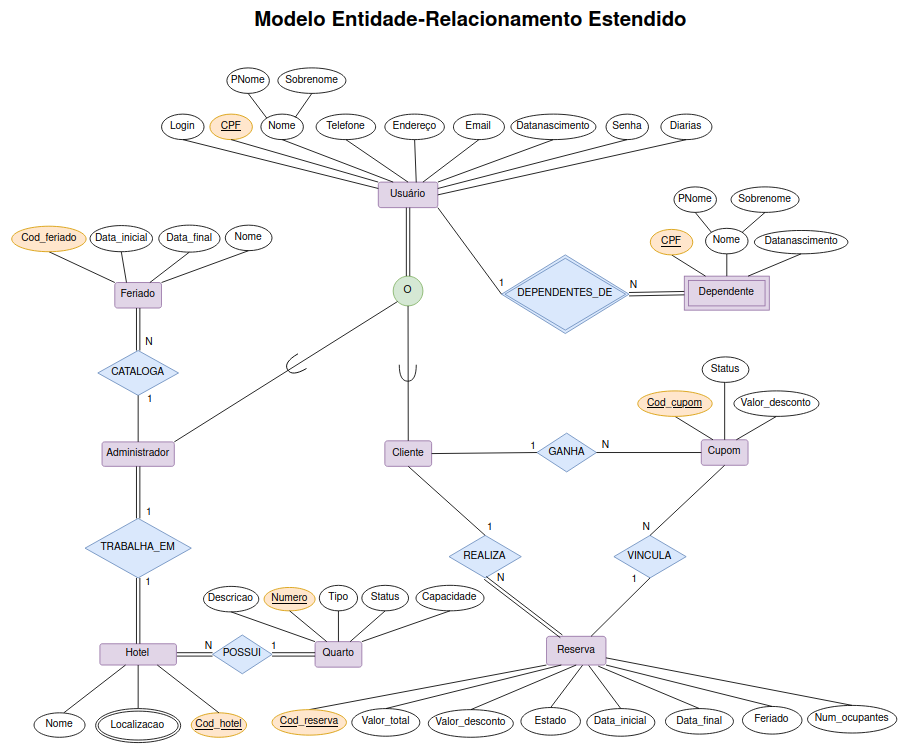
\includegraphics[width=1.1\textwidth]{Images/EER.png}
    \label{fig:exampleFig1}
\end{sidewaysfigure}

\subsection{Modelo Relacional}

Nesta seção, será discutida a modelagem do modelo relacional para refletir o modelo EER recém explanado. O diagrama foi formulado utilizando o mesmo algoritmo já aplicado na primeira etapa, mas como algumas nuances relacionadas à adição e modificação de relacionamentos, além da criação de tabelas "extras" na identificação de dependências funcionais e normalização do banco de dados.

\subsubsection{Desenvolvimento}

Como base, partimos do passo 1 do algoritmo, mapeamento todas as entidades regulares (excetuando a especialização, que será explanada adiante neste relatório) em relações, incluindo todos seus atributos correspondentes. As entidades mapeadas no passo 1 foram as seguintes: Cupom, Feriado, Quarto, Reserva e Hotel.

Na próxima etapa, mapeamos as entidades fracas presente no modelo EER, incluindo todos seus atributos como no passo anterior, mas incluindo como atributo de chave estrangeira, a chave primária da entidade com que esta se relaciona. \emph{Dependente} foi a entidade fraca mapeada no passo 2, enquanto a relação de identificação mapeada foi \emph{DEPENDENTES\_DE}.

Em seguida, aplicamos o passo 3 do algoritmo, utilizando a técnica da chave estrangeira para mapear o relacionamento \emph{TRABALHA\_EM} entre Administrador e Hotel (FK em Hotel que aponta para a chave primária do Administrador - CPF do Usuário). Como ambas entidades possuem participação total, poderia ser utilizada a técnica de mesclagem de relações. Optamos por não explorá-la devido ao mapeamento de especialização em relação única aplicada às subclasses e superclasse existentes no modelo, o que julgamos que prejudicaria a interpretação geral da modelagem do banco.

No passo 4, para o mapeamento de todos os relacionamentos binários (\(1:N\)), utilizamos a técnica da chave estrangeira, colocando-a no lado \(N\) da relação. Os relacionamentos mapeados desta forma foram os seguintes: \emph{CATALOGA}, \emph{POSSUI}, \emph{VINCULA}, \emph{REALIZA} e \emph{GANHA}.

No passo 6, para o mapeamento do único atributo multivalorado presente no modelo EER, criamos uma nova relação (\emph{Localização\_Hotel}), combinando como chave primária o par: código de hotel (também assume o papel de chave estrangeira) e seu respectivo endereço.

Por fim, mas de grande relevância, utilizamos o passo \emph{8D} (classes sobrepostas - \emph{overlapping}) no mapeamento de especialização da entidade Usuário em Cliente e Administrador. Com isso, mesclamos a superclasse e as subclasses em uma única relação contendo os atributos de todas as mesmas, que possui como chave primária, a chave primária da superclasse (CPF de Usuário). Além disso, foram incluídos dois atributos de tipo de relação: \emph{tipo\_administrador} e \emph{tipo\_cliente}. São atributos do tipo \emph{Boolean} que terão como propósito central, identificar a especialização da relação.

Finalizada a aplicação do algoritmo, foram criadas duas tabelas, a primeira destas sendo \emph{Reserva\_Cupom}. A mesma foi adicionada com o intuito de possibilitar a criação de reservas que não possuam cupons vinculados, possuindo como chave primária o par: \{cod\_reserva, cod\_cupom\}, que também atuam como chaves estrangeiras individualmente referenciando cupons e reservas. 

Já a segunda tabela foi criada a partir da verificação da dependência funcional do atributo \emph{senha} em \emph{Usuário} em relação as chaves candidatas. Este não depende funcionalmente da chave primária \emph{cpf}, então foi necessário criar a tabela \emph{Login} para atingir a 2ª forma normal na tabela \emph{Usuário}. Os detalhes sobre as soluções aplicadas e as dependências funcionais envolvidas no restante do esquema serão detalhadas posteriormente neste documento, assim como a forma normal em que o banco de dados como um todo se encontra. 

A representação ilustrativa do modelo relacional é exibida na página \pageref{fig:exampleFig2} na Figura \ref{fig:exampleFig2}.

\begin{sidewaysfigure}[ht]
    \centering
    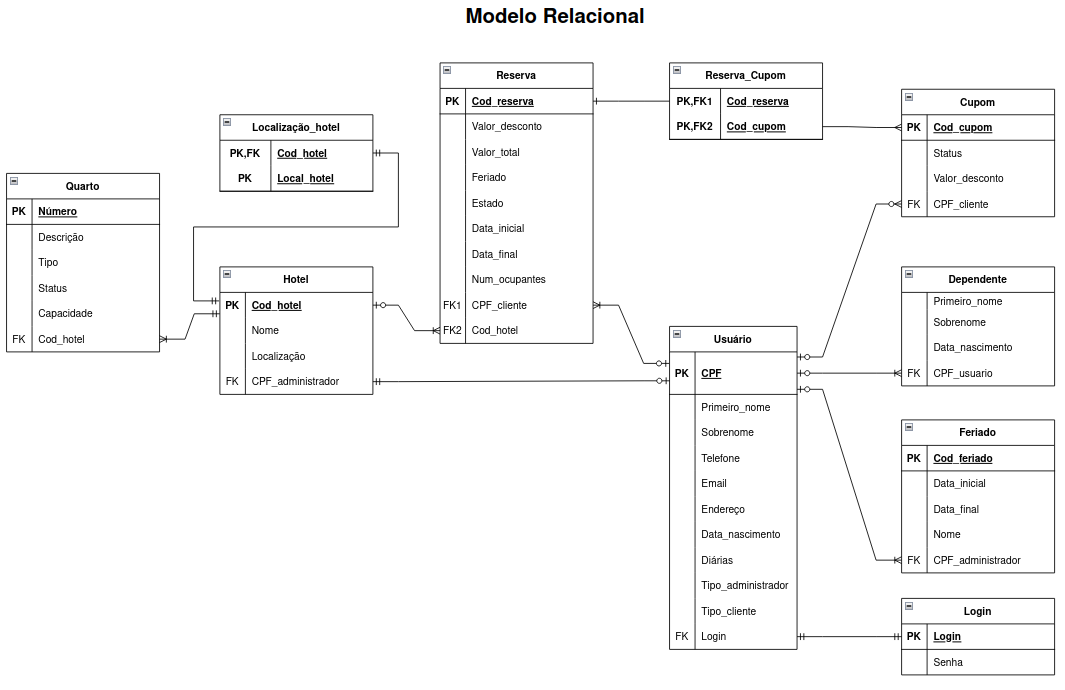
\includegraphics[width=1.1\textwidth]{Images/Relacional.png}
    \label{fig:exampleFig2}
\end{sidewaysfigure}

\section{Normalização}

Verificou-se que o atributo \emph{senha} pertencente a tabela usuário, não era dependente funcionalmente de todas as chaves candidatas da relação (e.g., em um cenário hipotético, vários usuários (cpf) podem possuir a mesma senha). Por isto, foi criada uma nova tabela (\emph{Login}), cuja chave estrangeira foi posicionada em usuário. Desta forma, nas duas tabelas em questão, quaisquer atributos são totalmente dependentes funcionalmente de todas as chaves candidatas.

Esta modificação permitiu o alcance da segunda forma normal, com todas as tabelas satisfazendo as mesmas definições formais. Embora tenhamos analisado brevemente níveis superiores de normalização, concluímos que esta é a forma normal máxima do banco no momento. Isto acontece porque existem tabelas cujos atributos não principais podem depender funcionalmente de atributos não principais de outras tabelas (e.g., o valor total de uma reserva depende do tipo de quarto), levando-nos a acreditar que o banco não está na terceira forma normal ou superior.

\section{Implementação}

A implementação do projeto foi realizada utilizando banco de dados \emph{MySQL}, juntamente com a ferramenta de interface gráfica cliente \textbf{MySQL Workbench 8.0} para efetuar as consultas SQL, administrar o sistema, modelar, criar e manter a base de dados por meio de um ambiente integrado. 

Para interagir com o banco de dados, foi escolhida a linguagem de programação \emph{PHP}, que possui como característica a facilidade para conexões com banco de dados. Para visualização no ambiente do cliente, utilizou-se o \emph{HTML}, linguagem de marcação utilizada na construção de páginas na \emph{Web}, e o \emph{CSS}, que possibilita estilização de um documento web, melhorando sua formatação e a visualização das informações.

Para configurar o banco de dados, em um primeiro momento foi utilizado o modelos conceituais, desenvolvendo assim, tabelas, relacionamentos, atributos, observando suas características e restrições. Após a primeira implementação, verificou-se a necessidade de uma revisão das tabelas e suas relações, para atender a ferramenta de normalização de banco de dados e as melhores práticas para seu desenvolvimento. Através da normalização e identificação das restrições e regras de negócio já estabelecidas, passou-se a desenvolver as páginas \emph{Web} para utilização dos recursos criados.

\subsection{Triggers}

Inicialmente, definimos uma \emph{Trigger} para realizar a checagem relacionada à usuários que atingem 20 diárias. Quando tal usuário satisfaz tal condição, este automaticamente ganharia 1 cupom de desconto de 10\%.

Uma \emph{Trigger} que atua como \emph{Assertion} relacionada a limitar o uso de cupons de 30\% ou mais em feriados prolongados também foi criada. Feriados com dois dias ou mais não permitem tal modo de utilização dos cupons.

A última \emph{Trigger} é reponsável pela checagem de cancelamento de um reserva realizada pelo usuário, o que automaticamente dispara uma ação para remover um cupom associado a tal usuário.

\section{Funcionalidades e Limitações}

As funcionalidades presentes resumem-se a cadastros, possibilitando a inserção de dados no banco para as tabelas correspondentes a usuário, hotel, reserva, quarto, feriado e cupom.

Foram implementados também algumas consultas para geração de relatórios, cuja principais funções são a apresentação dos resultados de consultas de interesse da administração do sistema. É importante citar que tais consultas só operam a nível de banco, ou seja, estas não estão integradas à interface do sistema. São exibidas algumas destas consultas nas Figuras \ref{fig:exampleFig3} e \ref{fig:exampleFig4}.

Como principais limitações, o sistema não implementa a navegação em ofertas sem que exista um \emph{login} ativo. Também não foram implementadas exclusões e as interações são realizadas de forma manual, além da ausência de um conjunto extenso de regras de negócio, principalmente relacionados as reservas.

\begin{figure}[H]
    \centering
    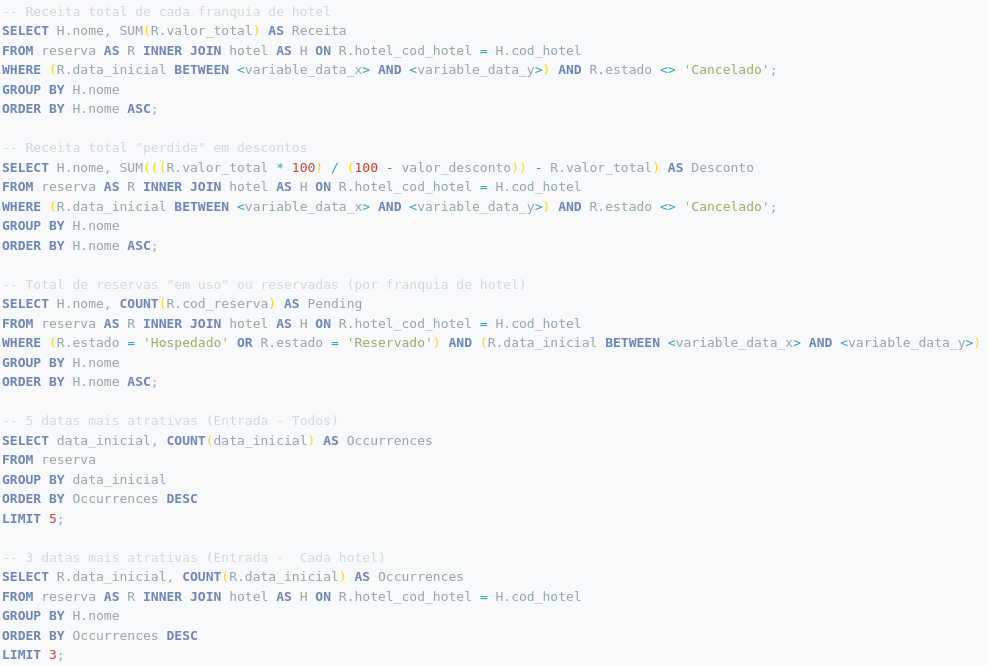
\includegraphics[width=1.2\textwidth]{Images/1.png}
    \label{fig:exampleFig3}
\end{figure}

\begin{figure}[H]
    \centering
    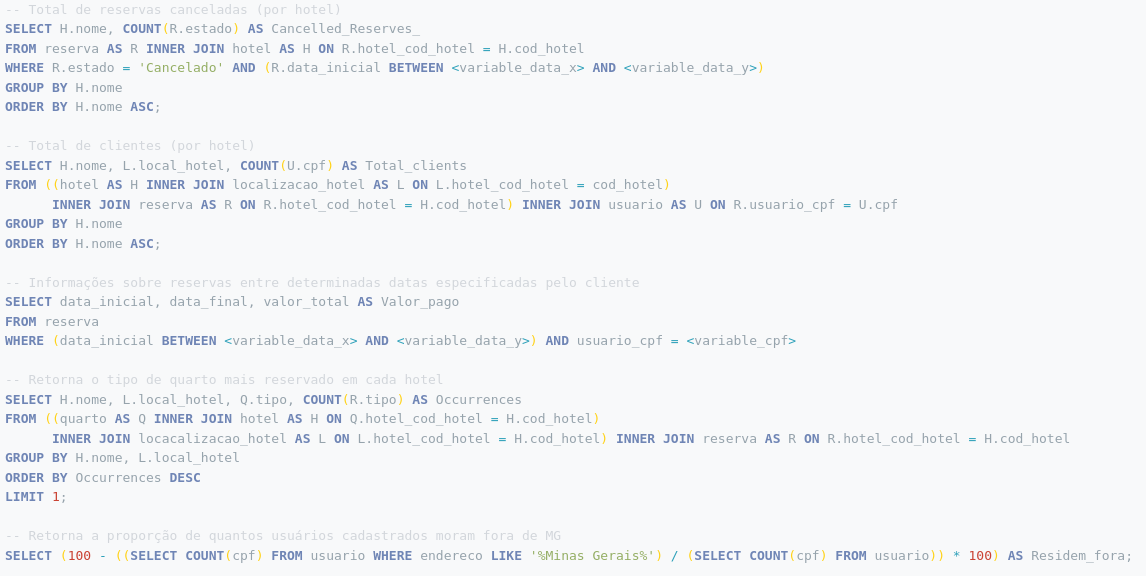
\includegraphics[width=1.15\textwidth]{Images/2.png}
    \label{fig:exampleFig4}
\end{figure}

\section{Conclusão}

Neste trabalho, experienciamos na prática, como é lidar com as dificuldades de um sistema completo envolvendo Banco de Dados, desde o \emph{Front-end} até o \emph{Back end}, utilizando diferentes ferramentas relacionadas. Os estudos realizados foram muito agregadores, uma vez que ajudaram no desenvolvimento e na compreensão dos principais conceitos vistos na teoria ministrada em aula. Além disto, foi possível vivenciar as principais dificuldades e decisões para a construção e manutenção de um sistema como um todo, e compreender de forma superficial as atividades envolvidas no trabalho realizado por administradores de Banco de Dados.

\section*{Referências}

\begin{itemize}
    \item Sistemas de Banco de Dados - Navathe - 6ª edição
    \item Material disponível no portal didático da disciplina de Banco de Dados
\end{itemize}

\end{document}